\section{FKA Results}
\label{sec:fka}

\subsection{The operating point}

\begin{table}[t]\centering\small
\caption{The FKA operating point. Bits measured, not projected. Addressability and edit locality
carry the $N$ they were measured at, per the stale-constant rule (\S\ref{sec:method}).}
\label{tab:fka}
\begin{tabular}{@{}lr@{}}
\toprule
quantity & value \\
\midrule
entities & 2,000,000 \\
facts & 8,000,000 \\
bits per entity & 52 \\
bits/bit (int8), amortised & 0.3938 \\
bits/bit (int8), marginal & 0.4387 \\
bits/param, amortised & 3.15 \\
bits/param, marginal & 3.51 \\
compression at 100\% addressability & 42.7x \\
addressability, direct ($N=2{,}000$) & 99.88\% \\
addressability, composed ($N=2{,}000$) & 99.56\% \\
edit locality & 0.00e+00 \\
\bottomrule
\end{tabular}

\end{table}

At $N = 2$M entities and 8M facts with 52 bits per entity, FKA stores \textbf{3.15 bits per
parameter amortised} and \textbf{3.51 marginal} (0.3938 / 0.4387 bits per bit, int8), with
\textbf{99.9\%} addressability and edit locality \textbf{0.00e+00}.
% experiments/2026-08-04_frontier/plot_data.json | M3 §24.5, §30
The gate is an operating point rather than a best-of: reporting the best capacity and the best
addressability from different configurations would describe no system.

\scope{The go/no-go split --- never-supervised 99.81\%, direct 99.88\%, composed 99.56\% --- was
measured at $N = 2{,}000$ (\texttt{experiments/2026-08-02\_m3-gonogo/gonogo.json}). The 99.9\%
headline is the $N = 2$M figure. The two are not interchangeable and the table labels each.}

The ceiling in this world is 0.296 asymptotically, and $>0.5$ bits per bit is unreachable here at
any $N$. That is \emph{corpus arithmetic, not architecture}: address cost grows as
$2.38\log_2 N$ while corpus entropy grows as $0.25\log_2 N$ (Proposition~\ref{prop:entropy}).

\subsection{Compression and structure}

Addressability holds at \textbf{100\%} down to 48 bits per fact --- a \textbf{42.7$\times$}
compression --- and \textbf{99.8\%} at 32 bits, at reconstruction cosine 0.82.
% experiments/2026-08-02_m3-sweep | M3 §11.5
The ordering that matters is \emph{structure beats residual per bit}: four quantisation stages with
\emph{no} residual (32 bits) reaches 99.8\%, while one stage plus an 8-dimensional residual
(72 bits) reaches only 82.3\%. More bits, worse addressability.

An early observation worth carrying: \textbf{addressability survives a 46\% relative reconstruction
error intact}. The encoder $f$ needs the part of the code that \emph{separates} entities, not the
code itself.
% M3 first point

\subsection{Degradation surfaces}

\begin{figure}[t]\centering
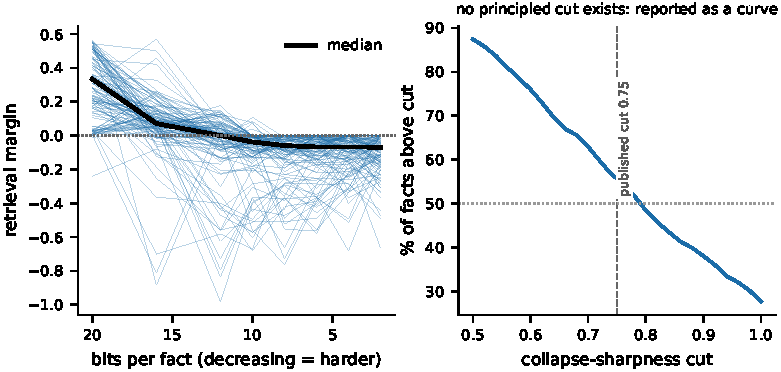
\includegraphics[width=0.98\linewidth]{figures/F4_margins}
\caption{Left: per-fact retrieval margin across the compression ladder (120 of 788 trajectories
drawn; median in black). Right: the fraction of facts above a collapse-sharpness cut, reported as a
\emph{curve} because no principled cut exists --- the published 0.75 is marked, and ``predominantly''
flips at 0.790. Both panels are computed from the persisted per-fact matrix, not from a summary.}
\label{fig:margins}
\end{figure}

The shape question --- attractor basins (plateau-then-cliff) against superposition (smooth decay) ---
was instrumented by the per-fact decode-quality \emph{distribution}, because the mean provably cannot
distinguish them. Two halves of the verdict have different standing, and the paper separates them.

\emph{Threshold-free and robust:} median collapse sharpness \textbf{0.790} against a uniform-slide
reference of \textbf{0.143} --- a factor of \textbf{5.5} --- and only \textbf{0.9\%} of facts
slide-like under a \emph{derived} criterion ($2/n_{\text{steps}}$). Smooth decay is excluded.

\emph{Threshold-dependent:} the widely-quoted ``55.8\% cliff-like'' depends on a cut of 0.75 that no
experiment produced. Sweeping it gives 87.4\% at 0.50 falling to 27.7\% at 1.00, and the word
``predominantly'' flips at \textbf{0.790} --- 5.4\% from the value chosen.
% M5 §5.126
The share above any cut is therefore reported as a curve (Figure~\ref{fig:margins}, right).

\scope{Only 1.5\% of trajectories are monotone, so the statistic's upper tail measures wobble rather
than sharper cliffs; the median and the slide-like fraction carry the verdict.}

A confound in the same data was broken without retraining: the apparent ordering by relation class
is \textbf{hop depth}, not relation type. With depth fixed, relation type barely matters (81.0\% vs
83.2\% at 16 bits); with relation fixed, depth matters enormously ($41.0\% \to 3.8\%$).
% M3 §12

\subsection{Address-cost scaling}

The minimum bits per entity for $\ge 99\%$ addressability was measured on nine corpus sizes from
2{,}000 to 2M, giving $2.38\log_2 N + 1.69$. A power form fits marginally better
(RMS 1.97 vs 2.06) and \emph{the discrimination does not resolve}: a 4.5\% residual gap on a 4-bit
ladder whose own scatter is $\pm 4$ bits is noise. Both forms predict within one ladder step of the
measured 52 bits at 2M and both put gate failure between 2.4M and 3.2M entities, so the
choice changes no decision --- which is the reportable fact.
% M3 §31

\scope{Searchability is honestly split and reopened as a standing item. Two-stage search restores
99.2\% entity recovery at $N = 2{,}000$, but recovery@1 falls to 59.3\% at 2M over clean codes and
99\% is unreachable at any shortlist size. The cause is \textbf{crowding}, not reconstruction noise,
and it is the larger bill; IVF is the only registered candidate and is priced, not run.}
% M2 §17

\subsection{Invariance under seeds}

Across ten seeds, FKA addressability shows $\sigma = \textbf{0.00}$ at \emph{five of seven}
compression rungs including the operating point, and $\sigma = \textbf{3.20}$ at its own
transition.
% experiments/2026-08-04_fka-seed-sweep | M5 §5.131

The sweep's design is itself a methodological point. A first probe at the operating point returned
100.0\% with zero variance --- saturated --- and comparing that against a dense spread measured
\emph{at a transition} would have been a comparison between incomparable regimes. The sweep was
moved onto the compression axis so both sides are measured where their own transitions are.
% M5 §5.131.1

\scope{The FKA seed varies \emph{store fitting and evaluation sampling}; the dense seed varies
\emph{model initialisation and training}. Both are run-to-run spread at a fixed configuration, and
they are not the same operation. This is stated as content, not as a weakness: no FKA
training-variance experiment exists, and none is claimed.}
